\section{Retrieve Process Implementation}
This section gives an overview of the architecture of the retrieve process which would restore the data back to the active
system from the Synology, so that it can be used for running more simulations and analyze the results. 

Figure \ref{fig:restoreClass} illustrates the class diagram for the retrieve process. The structure for the order of retrieve is very similar to the archive process
since it has to follow the MARS resource hierarchy (Section \ref{subsection:MARSResource}). All the dependencies for the retrieve project class are injected
using the Dependency Injection Container of ASP .NET framework. The restoring is done by getting the data from the Synology and then posting it back to the system
using the respective service.

\subsection{Addition of Functionalities in Other Services}
The restore needs to call many endpoints to upload the respective resource. After analyzing the MARS cloud and their available endpoints, it was
seen that some functionalities, which are needed for restoring the complete system, are not present in the current system. These functionalities are
added to the services for a successful restore. Table \ref{table:funcRestore} describes the functionalities that have been
added to the required services.

%\begin{table}[]
    %\centering
    \begin{longtable}{|p{2cm}|p{6cm}|p{6cm}|}
        \hline
            \textbf{Service}  & \textbf{Functionality} & \textbf{Description}\\
        \hline
            Project service & Add archived and is being archived mark in the project &  The archived mark is necessary because
            it would provide the user information if the queried project, is already archived, or is in the process of archiving. This has to be
            implemented using a GRPC communication, since this is the protocol in the project service, compared to the other services.  \\
        \hline
            Scenario service & Return scenario id with the full scenarios & It is the case when a full scenario is requested the scenario id is
            not returned. The id is required while retrieval because the service needs to map the old scenario id with the new one. If the mapping
            fails the simulation plans cannot be created since they are dependent upon scenarios.\\
        \hline
            Sim runner service & Upload a simulation run without running a simulation & The Sim-runner service executes the simulation run producing an
            output (simulation result) when it is created. This is not desired by the Archive service because a simulation result is already available that needs to be restored.
            Therefore, an added 
            functionality which uploads the simulation runs without running a simulation is implemented.\\
        \hline
            Database utility service & Dump and restore for result database & The simulation results are significantly large, so it is faster to
            perform a database dump for this. The dump and restore functionality is added, so that the archive service can restore and archive the simulation results.\\
        \hline
            Database utility service & Make the dump and restore a background job & It is crucial that the dumping and restoring process is implemented as a background task
            because this process is time-consuming in comparison to the other resources, i.e., scenario.\\

        \hline
        \caption{Functionality implemented to the other services for retrieve process}
        \label{table:funcRestore} 
    \end{longtable}

\begin{figure}[H]
    \centering 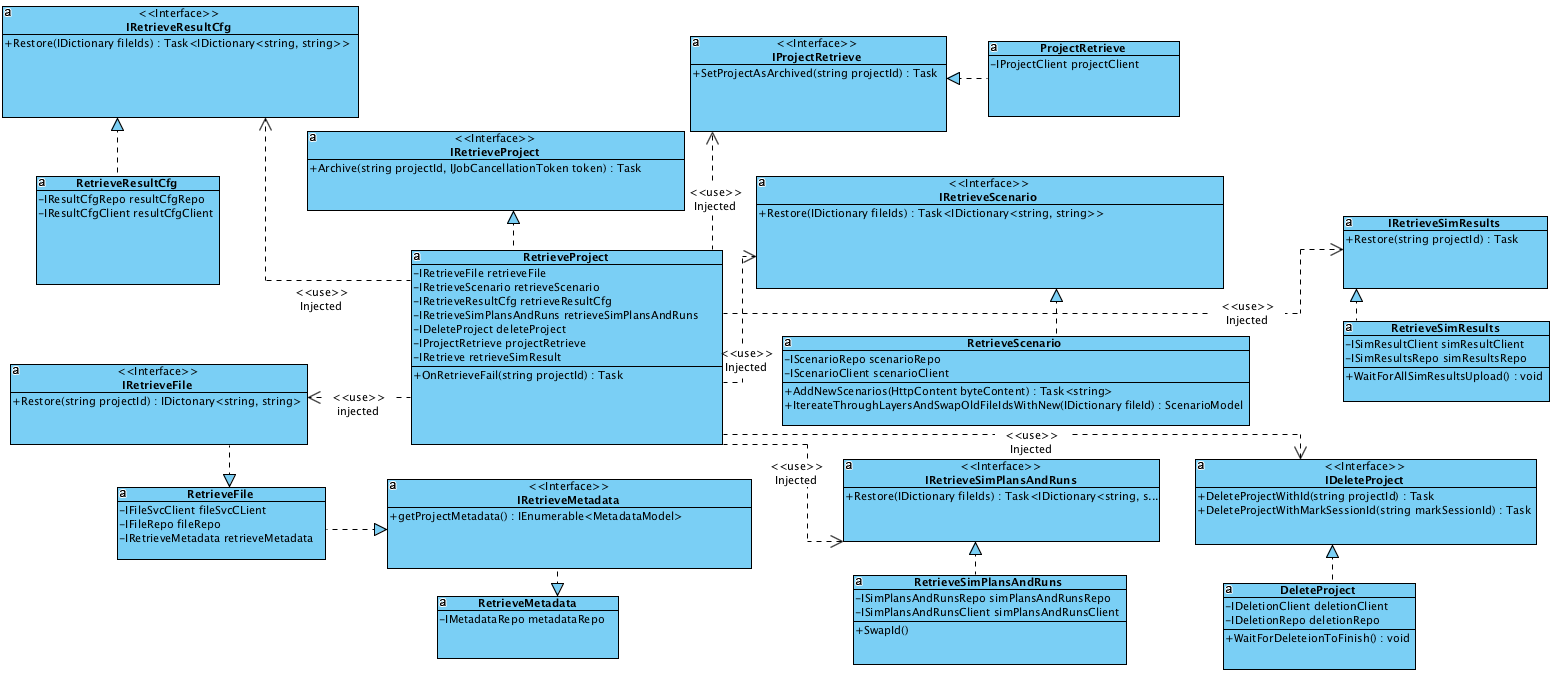
\includegraphics[height=6cm, angle=90, origin=c, width=10.5cm]{grafiken/restoreClass.png}
    \caption{Class Diagram for the Restore process (Top level)}
    \label{fig:restoreClass}
\end{figure}
